\begin{figure*}[t]
\centering
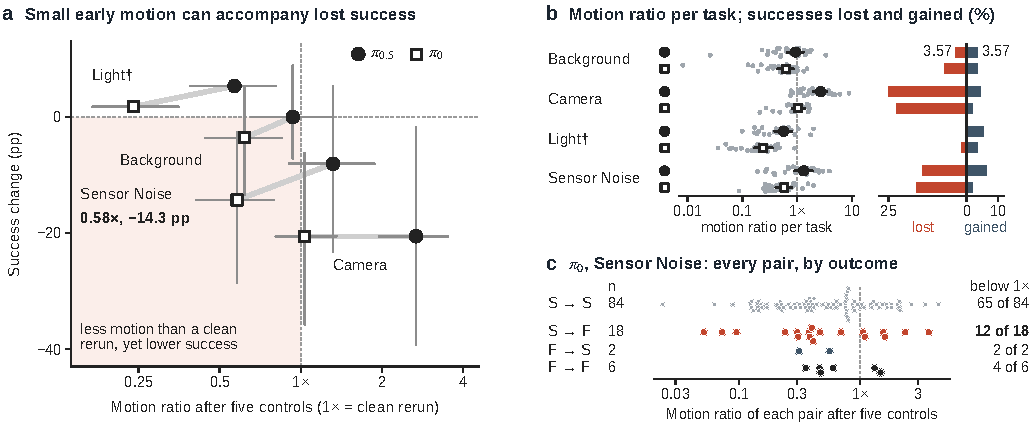
\includegraphics[width=\textwidth]{revised_figures/figure5_outcomes_v3.pdf}
\caption{\textbf{A small motion change can cost success, and net success hides lost and gained successes.} Unedited policies, 28 common tasks. Motion ratio: distance between a perturbed run and its clean run after five controls, relative to the distance between two clean runs (1$\times$: as far as a clean rerun). (a) Motion ratio of each family (95\% interval) against its change in success (98.75\% interval, i.e., 95\% Bonferroni-adjusted over four families); grey bands join the two policies of a family. In the shaded region a perturbation moves the robot less than a clean rerun and still lowers success: under Sensor Noise, $\pi_0$ moves 0.58$\times$ and loses 14.3 percentage points. (b) Left: motion ratio of every task (grey dots) and each family (markers). Right: successes lost and gained; for $\pi_{0.5}$ under Background both are 3.57\%. (c) All 110 $\pi_0$ Sensor Noise pairs by outcome (S, success; F, failure; clean$\to$perturbed), each relative to its own setting's clean rerun; the right column counts pairs below 1$\times$. Pairs that lose a success (S$\to$F) cover a similar range to pairs that keep it (S$\to$S). \dag\,For Light, some outcomes were not recorded: its marks use recorded outcomes only and carry no success interval, and its motion covers 43/48 settings on 26 tasks ($\pi_{0.5}$) and 44/48 on 27 ($\pi_0$). Bounds: Supplement, Sec.~S6.}
\label{fig:behavior}
\end{figure*}
